\documentclass[tikz,border=5pt]{standalone}
\usepackage{amsmath}
\definecolor{curveblue}{HTML}{245C86}
\begin{document}
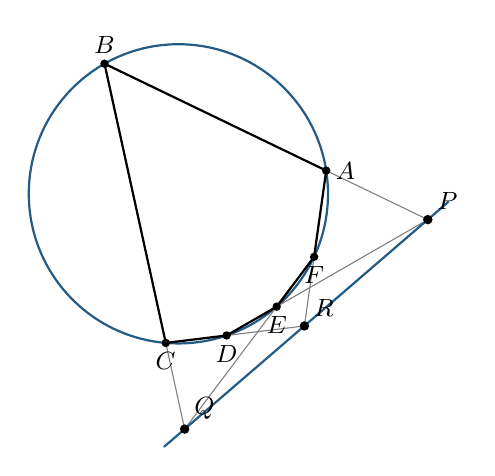
\begin{tikzpicture}[scale=1.9,font=\small,line cap=round]
\draw[curveblue,thick](0,0)circle(1);
\coordinate(A)at(0.9878974,0.1551085);
\coordinate(B)at(-0.4937411,0.8696090);
\coordinate(C)at(-0.0843177,-0.9964389);
\coordinate(D)at(0.3223425,-0.9466231);
\coordinate(E)at(0.6568891,-0.7539872);
\coordinate(F)at(0.9069979,-0.4211352);
\coordinate(P)at(1.6669751,-0.1723676);
\coordinate(Q)at(0.0420232,-1.5722686);
\coordinate(R)at(0.8421638,-0.8829451);
\draw[gray](A)--(P)--(B);
\draw[gray](D)--(P)--(E);
\draw[gray](B)--(Q)--(C);
\draw[gray](E)--(Q)--(F);
\draw[gray](C)--(R)--(D);
\draw[gray](F)--(R)--(A);
\draw[thick](A)--(B)--(C)--(D)--(E)--(F)--cycle;
\draw[curveblue,thick](1.8033471,-0.0548828)--(-0.0943488,-1.6897535);
\fill(A)circle(.8pt)node[right]{$A$};
\fill(B)circle(.8pt)node[above]{$B$};
\fill(C)circle(.8pt)node[below]{$C$};
\fill(D)circle(.8pt)node[below]{$D$};
\fill(E)circle(.8pt)node[below]{$E$};
\fill(F)circle(.8pt)node[below]{$F$};
\fill(P)circle(.9pt)node[above right]{$P$};
\fill(Q)circle(.9pt)node[above right]{$Q$};
\fill(R)circle(.9pt)node[above right]{$R$};
\end{tikzpicture}
\end{document}
